\documentclass[11pt,twoside,hidelinks]{book}

\usepackage[english]{babel}

% Font and spacing
\usepackage[scaled]{helvet}
\renewcommand\familydefault{\sfdefault}

% appendix stuff
\usepackage[toc,page]{appendix}

%\usepackage[hmarginratio=1:1]{geometry} %In case of twoside option: Same margins
\usepackage[a4paper,bottom=2.7cm]{geometry}
\savegeometry{mygeom}
\usepackage{cmap}
\usepackage[T1]{fontenc}
\usepackage[plain]{fancyref} % Fancy references, only have to use /ref, no "figure...". plain=no information on which page, otherwise: vario

% Change identation
\setlength\parindent{0pt}	% No identation after enter
\setlength\parskip{8pt}	% No identation after enter

% Change distance between items
\usepackage{enumitem}
% \setlist[1]{itemsep=-5pt}

% hyphenation
\tolerance=1
\emergencystretch=\maxdimen
\hyphenpenalty=10000
% \hbadness=10000

\usepackage{float}

\usepackage{listings}

\usepackage{subcaption}
\usepackage{wrapfig}
\usepackage{xr} %Cross Referencing

\usepackage[doublespacing]{setspace}

\usepackage{lipsum}

\usepackage{amsmath}
\usepackage{amssymb} % e.g for \lesssims
\usepackage{amsfonts}
\usepackage{bm} %  \bm for bold formatted symbols
\usepackage{graphicx}
\usepackage{url}
\usepackage{relsize}

\usepackage{pdfpages}   % Include pdf file

\newcommand*{\place}[1]{\gdef\@place{#1}}
\newcommand*{\supervisor}[1]{\gdef\@supervisor{#1}}

\addtocontents{toc}{\protect\thispagestyle{empty}} %No page number in contents

% Chapter page in fancyhdr has no page number
\usepackage{etoolbox}

% Nice and fancy stuff
\usepackage{xfrac}

% header
\usepackage{fancyhdr}
\pagestyle{fancy}% muss vor \renewcommand{\sectionmark} stehen
\setlength{\headheight}{13.6pt}
\renewcommand{\chaptermark}[1]{\markboth{#1}{}}
\fancyhf{} % Clears all page headers and footers
\fancyhead[LE,RO]{\leftmark}

\fancyhead[RE,LO]{\chaptername~\thechapter}
\fancyhead[LE,RO]{\thepage}

% Remove header on empty pages
\usepackage{emptypage}

% Tools for editing process
\usepackage{lineno}	% line numbers
\usepackage[colorinlistoftodos,prependcaption,textsize=small]{todonotes} % notes, use \todo
\newcommand{\todoquestion}[2][]
{\todo[backgroundcolor=cyan, #1]{#2}}

\usepackage{changepage} % allows change of textwidth with \begin{adjustwidth}

\usepackage{blindtext}

% For printing
\usepackage[colorlinks=true,urlcolor=black,citecolor=gray,linkcolor=black,pdfpagelayout=TwoPageRight]{hyperref}

% For pdf
% \usepackage[colorlinks=true,urlcolor=blue,citecolor=blue,linkcolor=black,pdfpagelayout=TwoPageRight]{hyperref}

% bibliographie

\usepackage{csquotes}
\usepackage[
  backend=biber,
  bibstyle=apa,
  citestyle=authoryear,
  % backref=true
]{biblatex}
\addbibresource{references.bib}
\providecommand{\apashortdash}{-}

% \DeclareFieldFormat{apadate}{\mkbibparens{\printdate}.....}

% make autocite use also the year
\DeclareCiteCommand{\autocite}
  {\usebibmacro{prenote}}
  {\usebibmacro{citeindex}%
   \printtext[bibhyperref]{(\printnames{labelname}%
     \setunit{\addcomma\space}%
     \printfield{year}}}
  {\multicitedelim}
  {\usebibmacro{postnote})}

\usepackage[nottoc]{tocbibind} %Bibliography in toc
% \usepackage[noadjust]{cite} % 'sort' and 'compress' are enabled by default -> More than two citations are combined with a --

% Change format of backref
% \renewcommand*{\backref}[1]{}
% \renewcommand*{\backrefalt}[4]{{%
%     \ifcase #1 Not cited.%
%           \or Zitiert auf Seite~#2.%
%           \else Zitiert auf Seiten #2.%
%     \fi%
%     }}

%  makes brackets around equation references
\makeatletter
\let\oldtheequation\theequation
\renewcommand\tagform@[1]{\maketag@@@{\ignorespaces#1\unskip\@@italiccorr}}
\renewcommand\theequation{(\oldtheequation)}
\makeatother

% Colored checkmarks
\newcommand{\checkmarkRed}{{\color{red}\checkmark}}
\newcommand{\checkmarkOrange}{{\color{orange}\checkmark}}
\newcommand{\checkmarkGreen}{{\color{green}\checkmark}}
\newcommand{\exclamationRed}{{\color{red}\textbf{!}}}


% Table utilities
\usepackage{multirow}
\usepackage{makecell} % Use \makecell{Some really \\ longer text} to split cell
\usepackage{array}
\newcolumntype{H}{>{\setbox0=\hbox\bgroup}c<{\egroup}@{}} % Hide column by using \begin{tabular}{llHl} (H is hidden)

\usepackage{tabularray}   % search for the package for instructions on how to create tables

\makeatletter
\renewenvironment{titlepage}
 {%
  \if@twocolumn
    \@restonecoltrue\onecolumn
  \else
    \@restonecolfalse\newpage
  \fi
  \thispagestyle{empty}%
 }
 {%
  \if@restonecol
    \twocolumn
  \else
    \newpage
  \fi
 }
\makeatother

% for \bottomrule and similar
\usepackage{booktabs}

% Heading without numbering
\newcommand{\heading}[1]{\subsection*{#1} \vspace{-3mm}}

% big "C" in chapter etc
\renewcommand{\chapterautorefname}{Kapitel}
\renewcommand{\sectionautorefname}{Abschnitt}

% to strike text through using \sout
\usepackage[normalem]{ulem}

% Use certain pages in landscape (\begin{landscape} \end{landscape} \clearpage)
\usepackage{rotating}

% captions
\captionsetup[figure]{labelfont={bf},textfont={}, font=footnotesize}
\captionsetup[subfigure]{labelfont={bf},textfont={}, font=footnotesize}
\captionsetup[table]{labelfont={bf},textfont={}, font=footnotesize}

% Remove header until \pagestyle{fancy} is used again
\fancypagestyle{plain}{% copy pagestyle fancy
     \fancyhead[]{}% but remove all header fields
     \renewcommand{\headrule}{}}% and remove the headrule

% Itemize spacing
\usepackage{changepage}
% \let\tempone\itemize
% \let\temptwo\enditemize
% \renewenvironment{itemize}{\tempone\addtolength{\itemsep}{0.5\baselineskip}}{\temptwo}

% copy text
\makeatletter
\newcommand\remembertext[2]{% #1 is a key, #2 is the text
  \immediate\write\@auxout{\unexpanded{\global\long\@namedef{mytext@#1}{#2}}}%
  #2%
}

\newcommand\recalltext[1]{%
  \ifcsname mytext@#1\endcsname
    \@nameuse{mytext@#1}%
  \else
    ``??''
  \fi
}
\makeatother

% appendix tables
\DeclareFontFamily{\encodingdefault}{\ttdefault}{%
  \hyphenchar\font=\defaulthyphenchar
  \fontdimen2\font=0.33333em
  \fontdimen3\font=0.16667em
  \fontdimen4\font=0.11111em
  \fontdimen7\font=0.11111em
}

\begin{document}

\frontmatter % Use roman page numbering style (i, ii, iii, iv...) for the pre-content pages
\pagenumbering{Roman}     % large roman numbers
\newgeometry{hmarginratio=1:1}
\begin{titlepage}
    
\includepdf[pages={1},pagecommand={}]{others/your_titlepage.pdf}
\end{titlepage}
\restoregeometry{}

\chapter*{Abstract}\addcontentsline{toc}{chapter}{Abstract}\markboth{Abstract}{Abstract}

Describe your work.
\pagestyle{fancy}
\chapter*{Acknowledgements}\addcontentsline{toc}{chapter}{Acknowledgements}\markboth{DanAcknowledgementssagung}{Acknowledgements}

Thank you rmnmllr.

\pagestyle{fancy}
\renewcommand{\chaptermark}[1]{\markboth{#1}{}}
\fancyhf{}
\fancyhead[LE]{\thepage}
\fancyhead[RE]{Inhaltsverzeichnis}
\fancyhead[LO]{Inhaltsverzeichnis}
\fancyhead[RO]{\thepage}

\renewcommand{\baselinestretch}{0.9}\normalsize
\tableofcontents
\renewcommand{\baselinestretch}{1.25}\normalsize

\mainmatter % Begin numeric (1,2,3...) page numbering
% \linenumbers

% Introduction
\pagestyle{fancy}
\fancyhf{}
\fancyhead[LE]{\thepage}
\fancyhead[RE]{Einleitung}
\fancyhead[LO]{Einleitung}
\fancyhead[RO]{\thepage}
\chapter*{Introduction}\label{ch:introduction}\addcontentsline{toc}{chapter}{Introduction}\markboth{Introduction}{Introduction}

An introduction to your work.

This is how to textcite with APA style: According to \textcite{muller_github_2023} this is a template.

And this is how to autocite: The template can be found on rmnmllr's GitHub \autocite{muller_github_2023}.

Compile your library in BibLatex format by hand (see references.bib) or using Zotero, Mendeley and any other tool.
\cleardoublepage

% Chapters
\renewcommand{\chaptermark}[1]{\markboth{#1}{}}
\renewcommand{\sectionmark}[1]{\gdef\rightmark{#1}}
\fancyhf{}
\fancyhead[LE]{\thepage}
\fancyhead[RE]{\chaptername~\thechapter: \leftmark}
\fancyhead[LO]{Abschnitt~\thesection:~\nouppercase{\rightmark}}
\fancyhead[RO]{\thepage}

\chapter{Xx} \label{ch:xx}

This is text for Chapter \ref{ch:xx}.
\cleardoublepage

\chapter{Yy} \label{ch:yy}

This is some text.
\begin{figure}[ht]
    \centering
    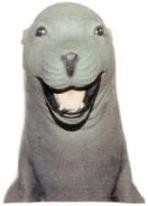
\includegraphics{figures/im_scratchyseal.jpg}
    \caption{An example image from the figures directory.}
    \label{fig:example}
\end{figure}
\cleardoublepage

% \backmatter

% Bibliography
\fancyhf{}
\fancyhead[LE]{\thepage}
\fancyhead[RE]{Literaturverzeichnis}
\fancyhead[LO]{Literaturverzeichnis}
\fancyhead[RO]{\thepage}

\printbibliography[
    heading=bibintoc,
    title=Literaturverzeichnis
]

\fancyhf{}
\fancyhead[LE]{\thepage}
\fancyhead[RE]{Abbildungsverzeichnis}
\fancyhead[LO]{Abbildungsverzeichnis}
\fancyhead[RO]{\thepage}
\listoffigures
\cleardoublepage

\fancyhf{}
\fancyhead[LE]{\thepage}
\fancyhead[RE]{Tabellenverzeichnis}
\fancyhead[LO]{Tabellenverzeichnis}
\fancyhead[RO]{\thepage}
\listoftables
\cleardoublepage

\fancyhf{}
\fancyhead[LE]{\thepage}
\fancyhead[RE]{Selbst\"andigkeitserkl\"aerung}
\fancyhead[LO]{Selbst\"andigkeitserkl\"aerung}
\fancyhead[RO]{\thepage}
\begin{figure}\addcontentsline{toc}{chapter}{Selbst\"andigkeitserkl\"aerung}\markboth{Selbst\"andigkeitserkl\"aerung}{Selbst\"andigkeitserkl\"aerung}
	\centering
	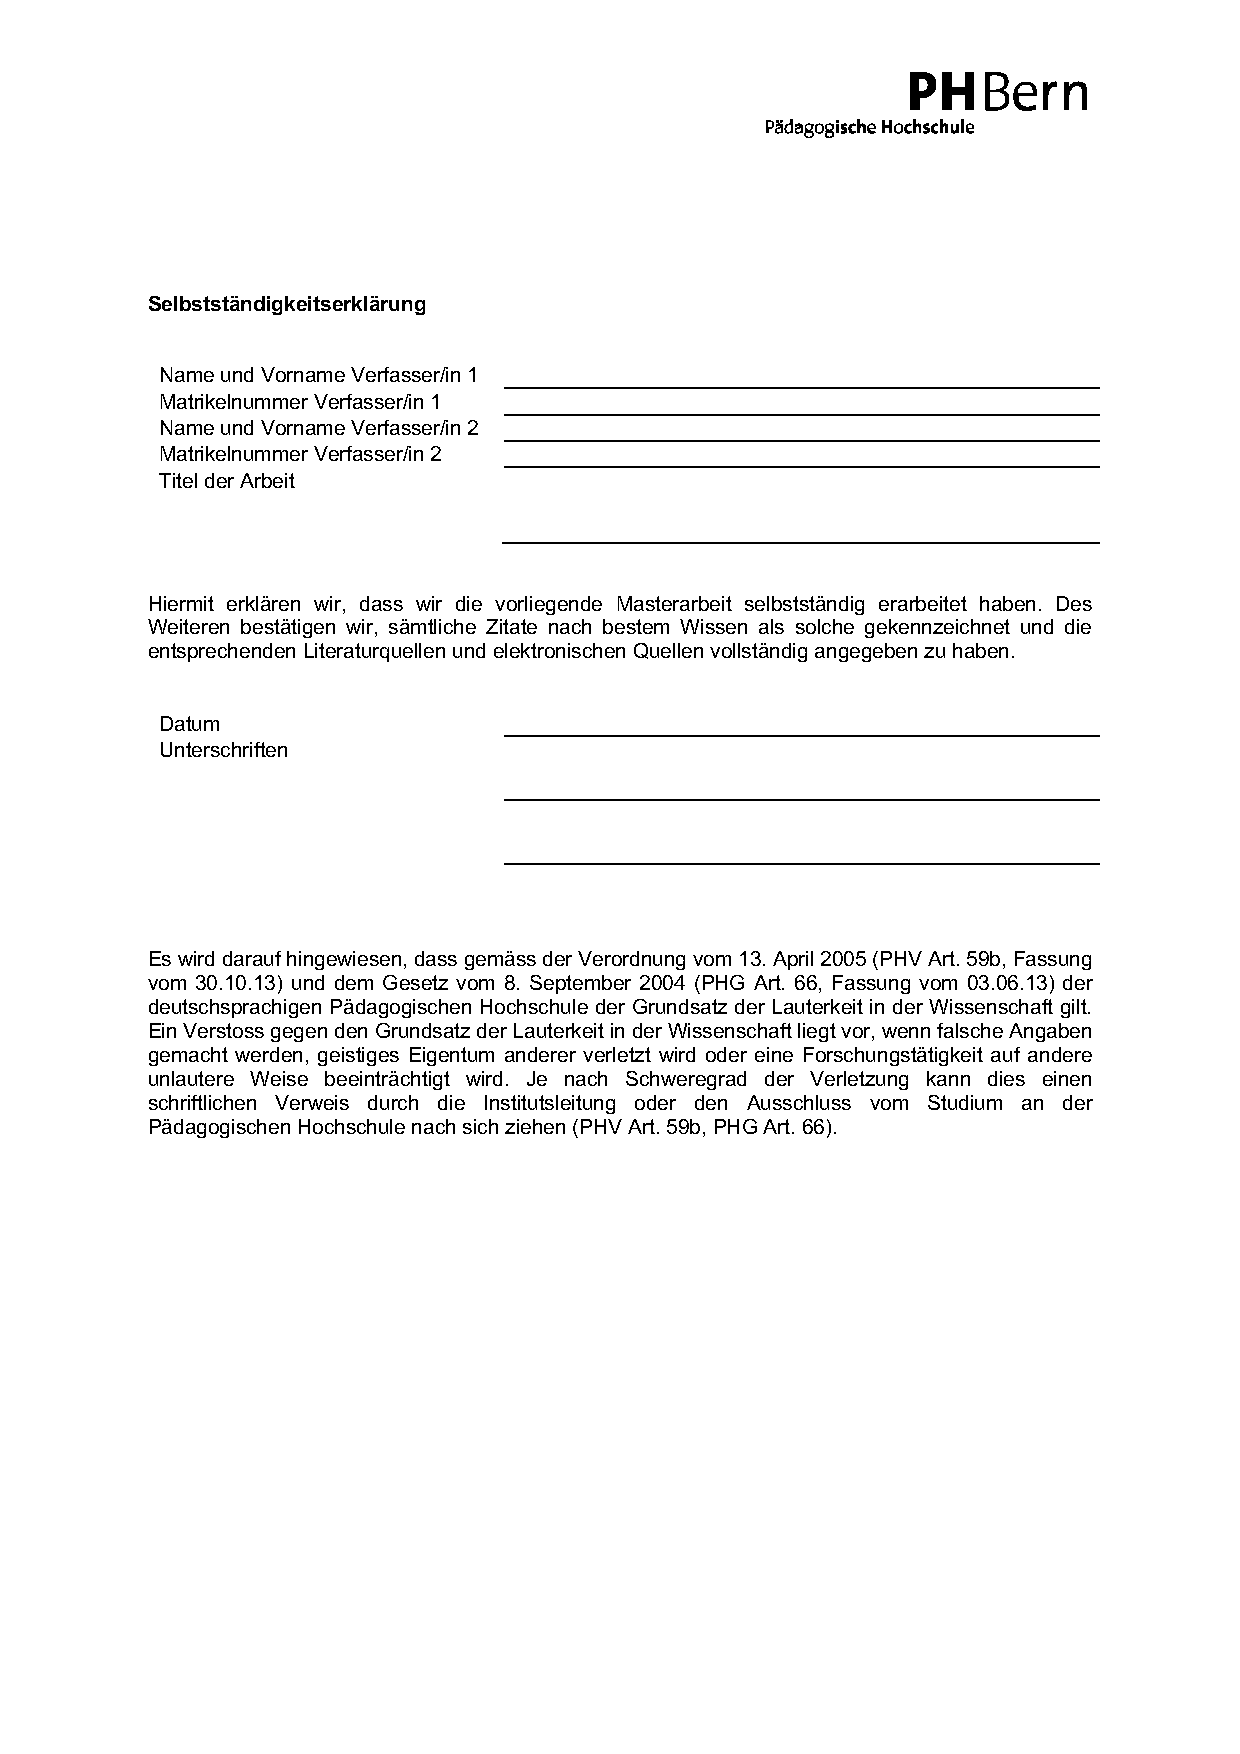
\includegraphics[page=1,height=\textheight]{others/declaration.pdf}
\end{figure}
\cleardoublepage

\appendix

\fancyhf{}
\fancyhead[LE]{\thepage}
\fancyhead[RE]{\chaptername~\thechapter: \leftmark}
\fancyhead[LO]{Abschnitt~\thesection:~\nouppercase{\rightmark}}
\fancyhead[RO]{\thepage}

\chapter{Some title}


\cleardoublepage

\end{document}

